\subsection{LSTM}


\begin{frame}{Long Short-Term Memory (LSTM)}

\begin{figure}[h]
\centering
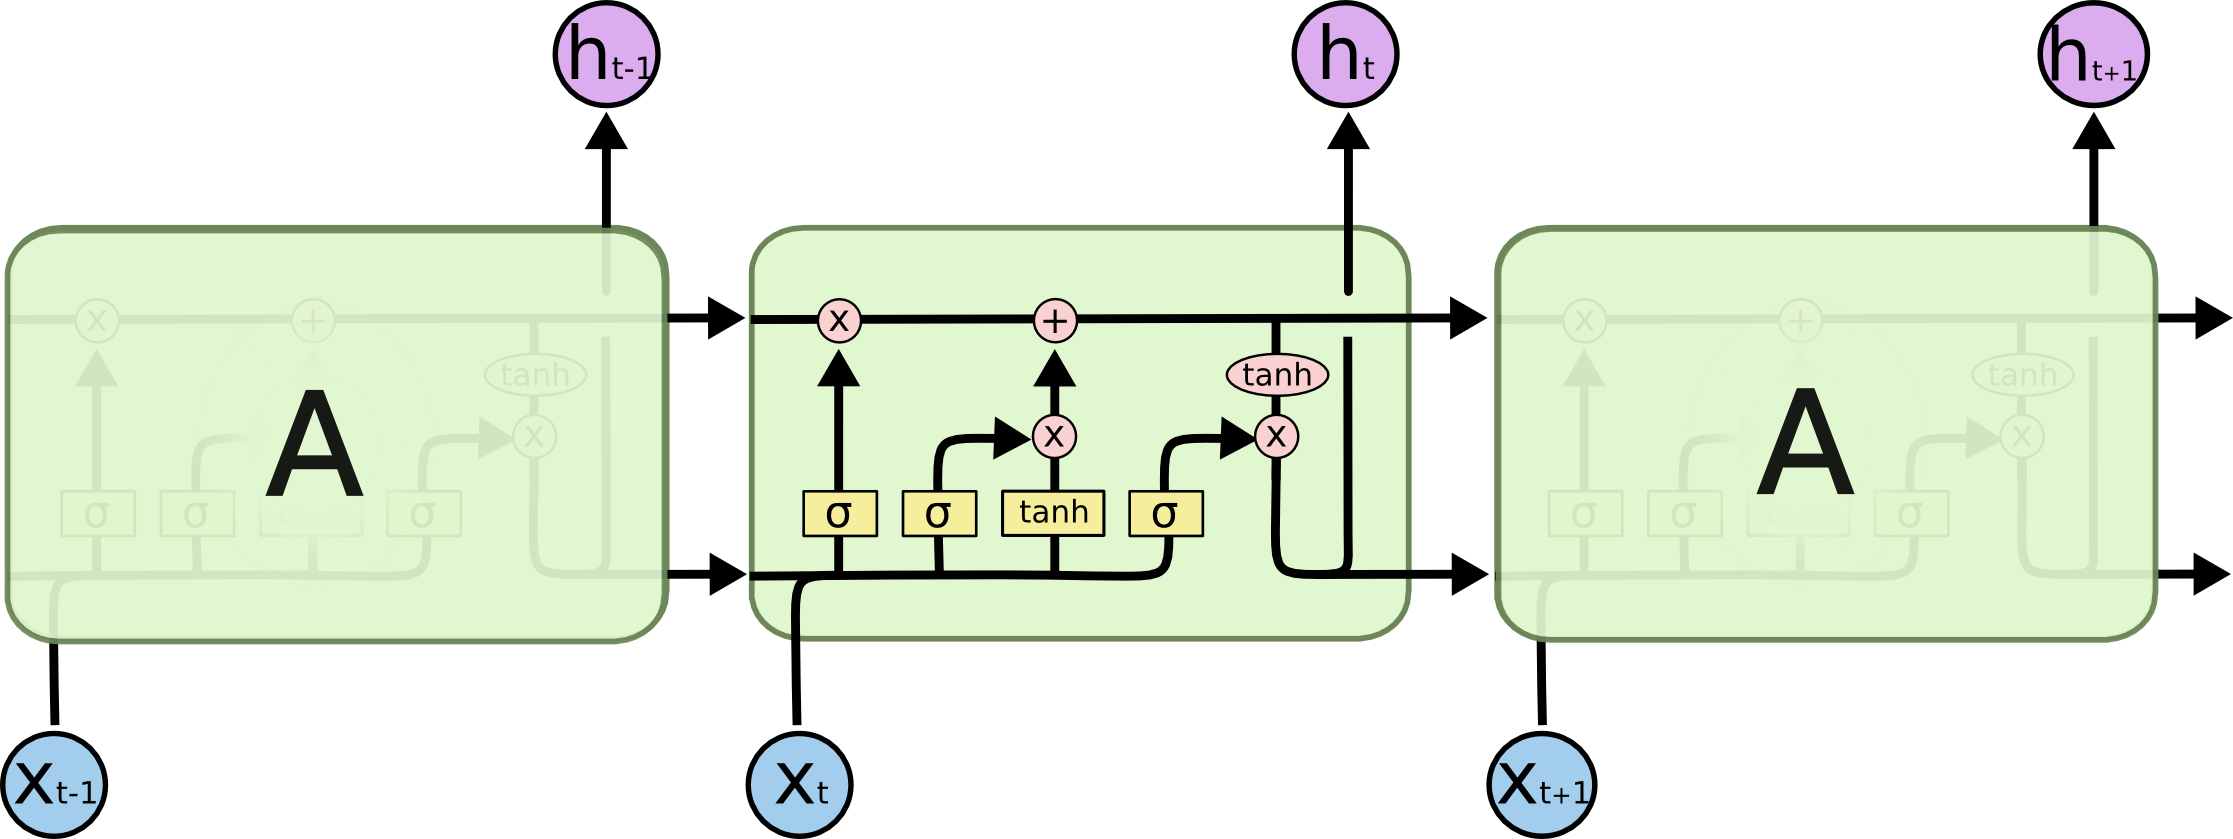
\includegraphics[width=1\textwidth]{fig/Olah_LSTM1.png}
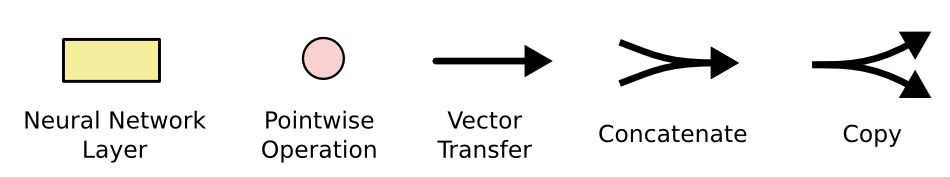
\includegraphics[width=1\textwidth]{fig/Olah_LSTM1b.png}
\caption{The LSTM (Olah, 2015)}
\end{figure}

\end{frame}


\begin{frame}{LSTM cell state}

\begin{figure}[h]
\centering
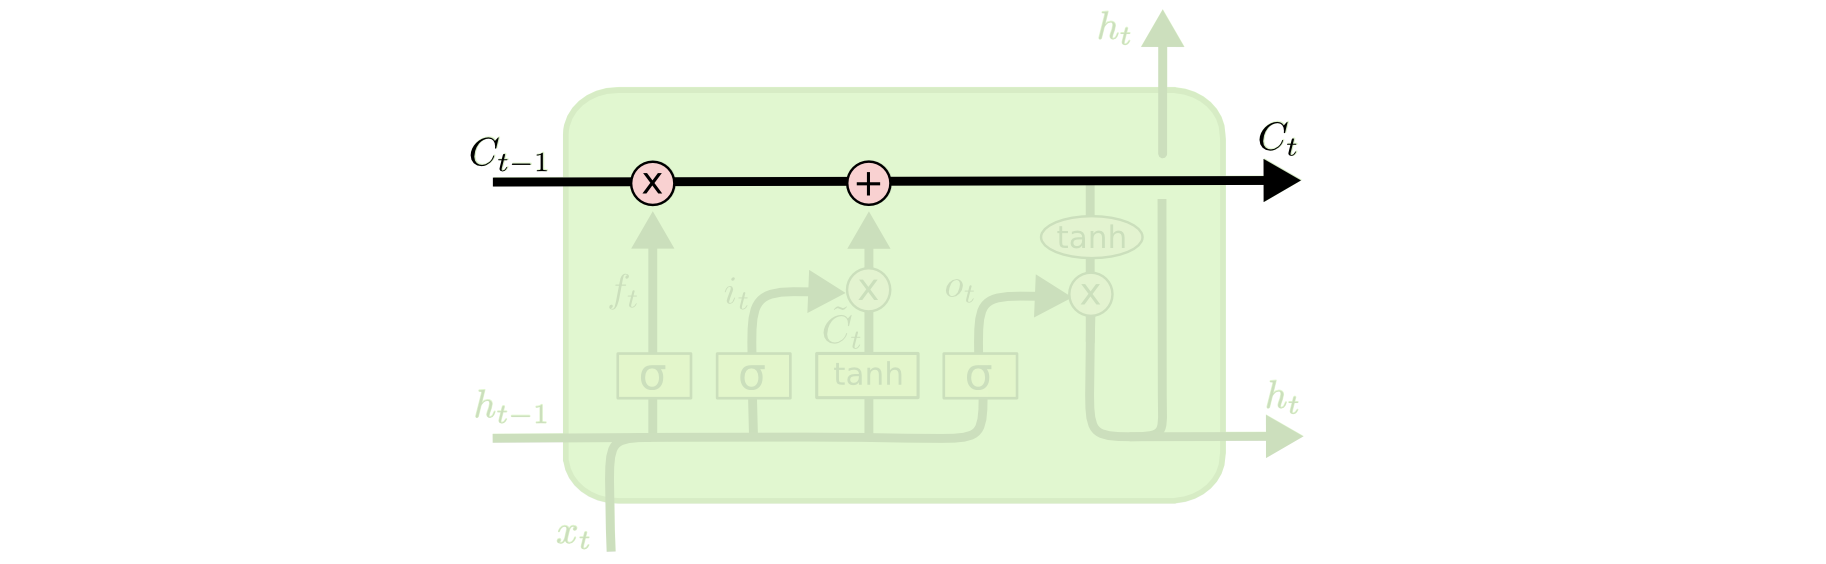
\includegraphics[width=1\textwidth]{fig/Olah_LSTM2.png}
\caption{LSTM cell state, i.e. "carrybelt" (Olah, 2015)}
\end{figure}

\end{frame}

\begin{frame}{LSTM forget gate}

\begin{figure}[h]
\centering
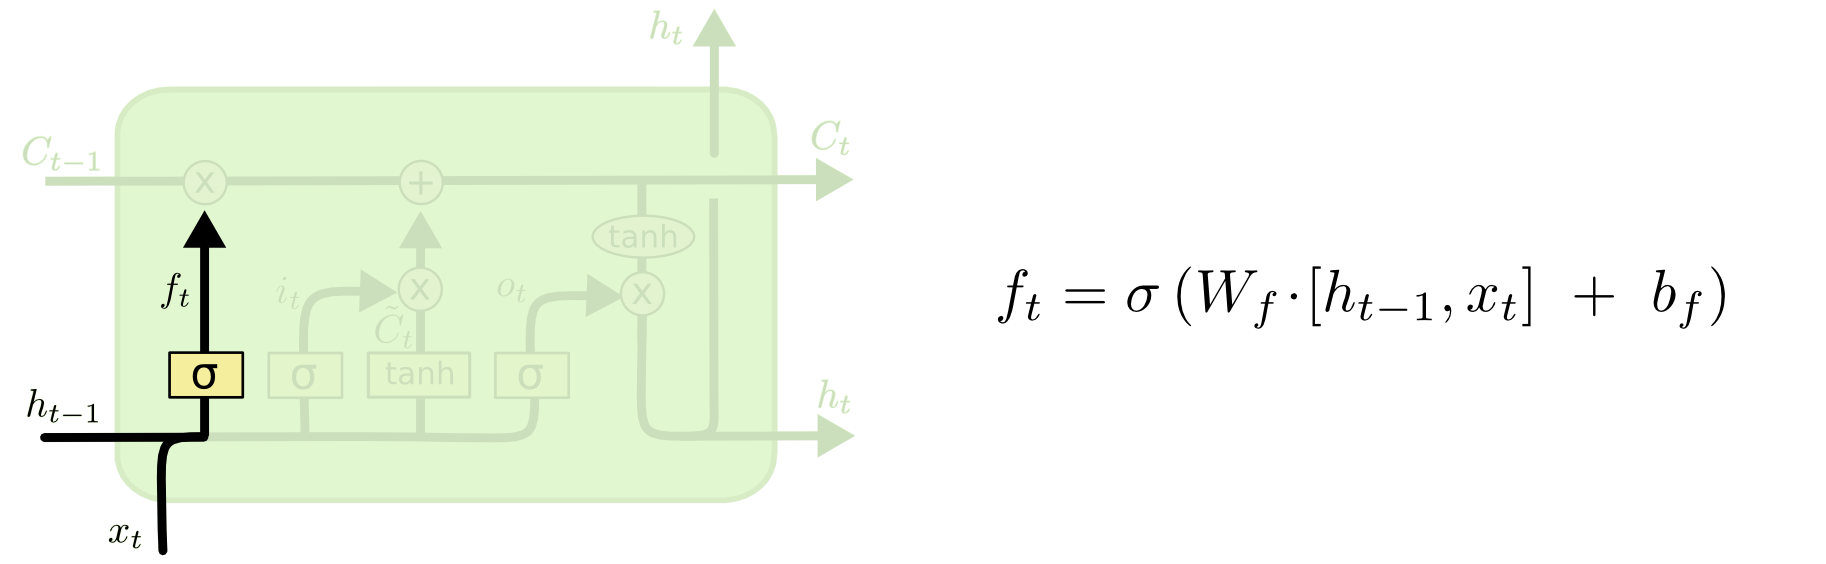
\includegraphics[width=1\textwidth]{fig/Olah_LSTM3_forget.png}
\caption{LSTM forget gate (Olah, 2015)}
\end{figure}

\end{frame}

\begin{frame}{LSTM input gate}

\begin{figure}[h]
\centering
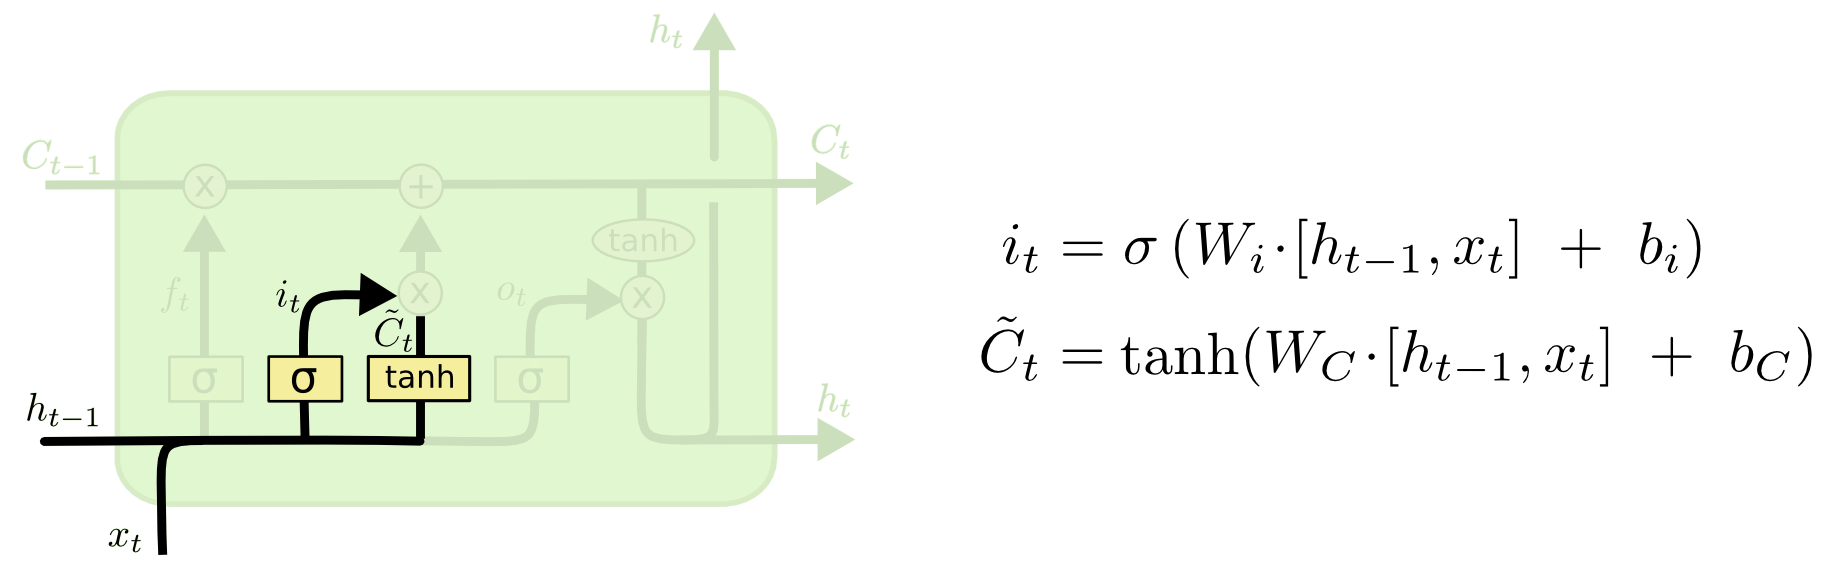
\includegraphics[width=1\textwidth]{fig/Olah_LSTM3_update.png}
\caption{LSTM input gate (Olah, 2015)}
\end{figure}

\end{frame}

\begin{frame}{LSTM cell state update}

\begin{figure}[h]
\centering
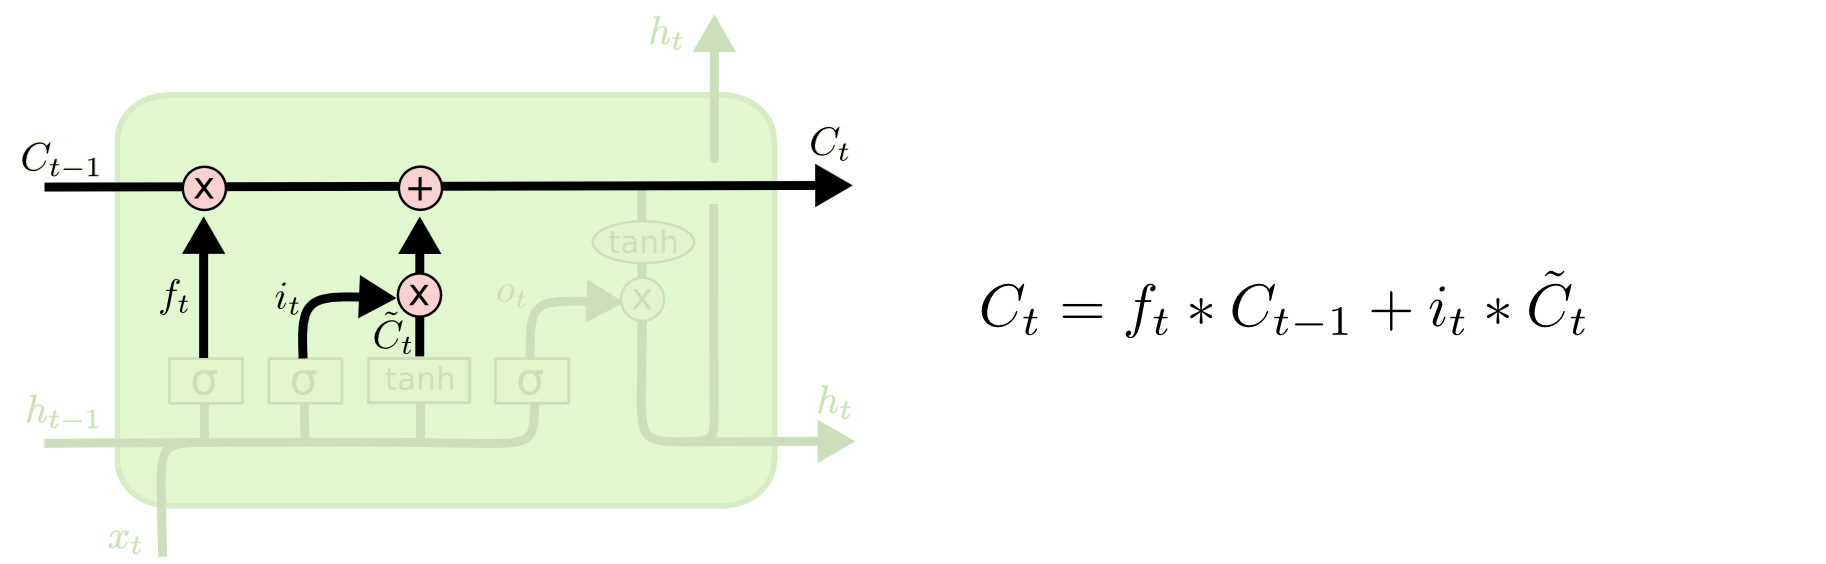
\includegraphics[width=1\textwidth]{fig/Olah_LSTM3_update2.png}
\caption{Update cell state (Olah, 2015)}
\end{figure}

\end{frame}

\begin{frame}{LSTM output gate}

\begin{figure}[h]
\centering
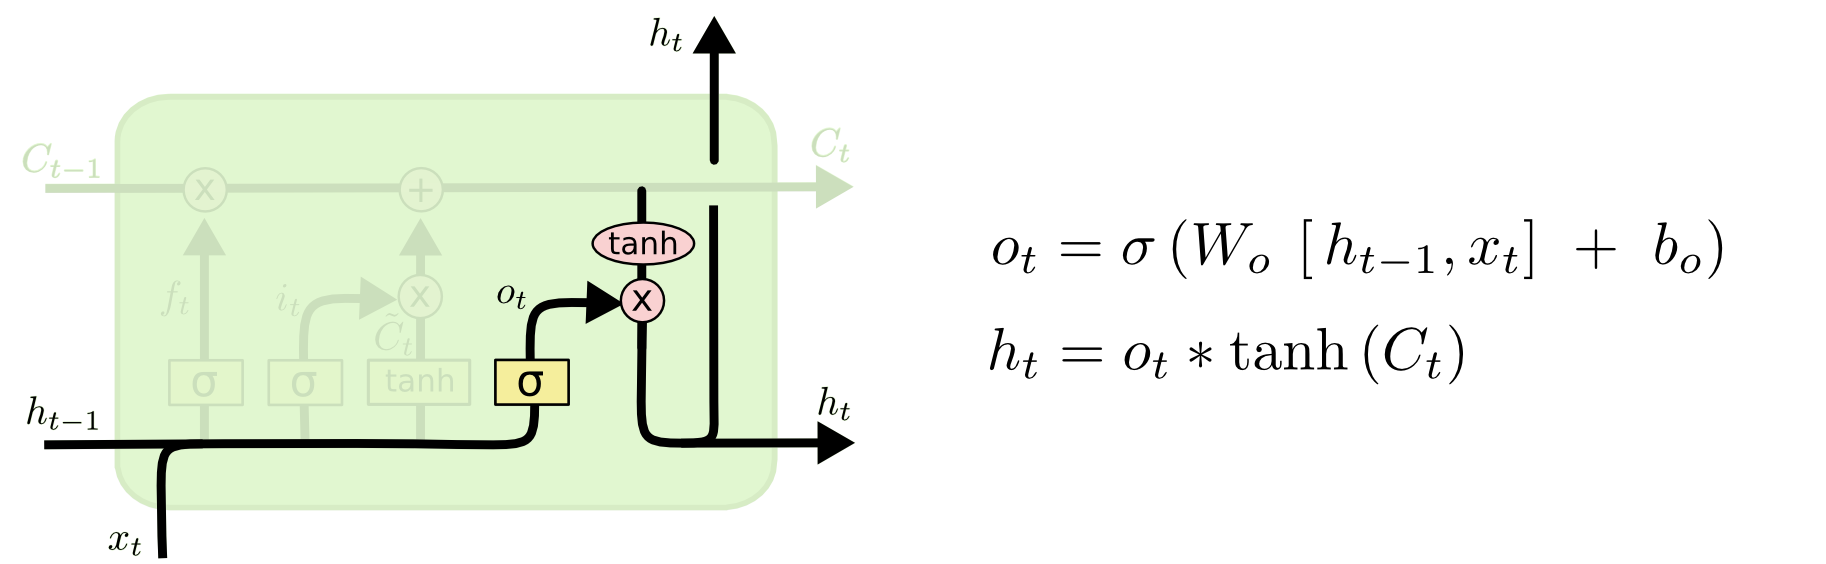
\includegraphics[width=1\textwidth]{fig/Olah_LSTM3_output.png}
\caption{LSTM output gate (Olah, 2015)}
\end{figure}

\end{frame}


\begin{frame}{Problems}

\begin{itemize}
\item Still a {\color{uured} recurrent structure},\\(vanishing and exploding gradients)
\item Long-term dependencies still difficult
\item Hard to do {\color{uured} transfer learning}
\end{itemize}


\end{frame}
